\section{Banach Spaces} 

	The idea is that we want to construct $L^p$ spaces and claim that it is a Banach space. 

  \begin{lemma}[Young's Inequality]
    \label{thm:youngs-inequality}
    Suppose $1 \leq p < +\infty$, with $q = \frac{p}{p-1}$, i.e. $\frac{1}{p} + \frac{1}{q} = 1$. Let $a, b \geq 0$. Then 
    \begin{equation}
      a b \leq \frac{a^p}{p} + \frac{b^q}{q} 
    \end{equation}
  \end{lemma}
  \begin{proof}
    Let the \hyperref[real-def:exponential-function]{exponential function} be $y = x^{p-1}$. Then, we get $x = y^{\frac{1}{p-1}}$. The proof is similar to if the function intersects the upper side of the rectangle. 

    \begin{figure}[H]
      \centering
      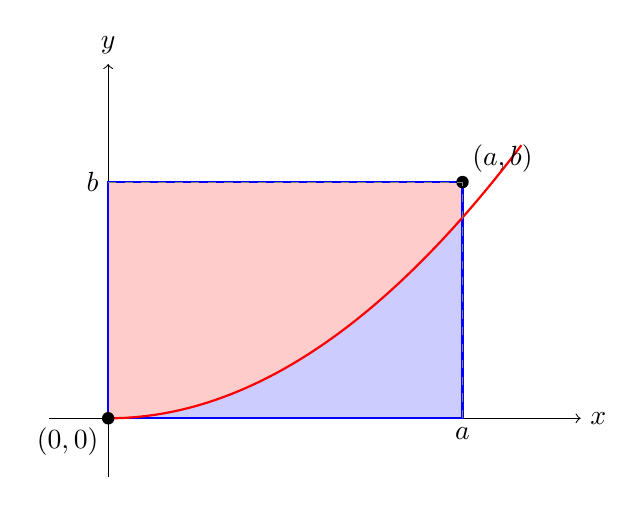
\begin{tikzpicture}[scale=1.5]
        % Draw axes
        \draw[->] (-0.5,0) -- (4,0) node[right] {$x$};
        \draw[->] (0,-0.5) -- (0,3) node[above] {$y$};
        
        % Define a and b
        \def\a{3}
        \def\b{2}
        
        % Shade area below the curve
        \fill[blue!20] (0,0) -- plot[domain=0:\a, samples=100] (\x, {1.7*(\x/\a)^2}) -- (\a,0) -- cycle;
        
        % Shade area above the curve
        \fill[red!20] plot[domain=0:\a, samples=100] (\x, {1.7*(\x/\a)^2}) -- (\a,\b) -- (0,\b) -- (0,0);
        
        % Draw rectangle
        \draw[blue, thick] (0,0) rectangle (\a,\b);
        
        % Draw exponential function extended beyond (a,b)
        \draw[red, thick, domain=0:3.5, samples=100] plot (\x, {1.7*(\x/\a)^2});
        
        % Label vertices
        \node[below left] at (0,0) {$(0,0)$};
        \node[above right] at (\a,\b) {$(a,b)$};
        
        % Mark points
        \fill (0,0) circle (1.5pt);
        \fill (\a,\b) circle (1.5pt);
        
        % Draw dashed lines to axes
        \draw[dashed, gray] (\a,0) -- (\a,\b);
        \draw[dashed, gray] (0,\b) -- (\a,\b);
        
        % Label axes values
        \node[below] at (\a,0) {$a$};
        \node[left] at (0,\b) {$b$};
      \end{tikzpicture}
      \caption{Rectangle with exponentially increasing curve and shaded regions}
      \label{fig:rectangle}
    \end{figure}

    We can see that the blue region has area 
    \begin{equation}
      \int_0^a x^{p-1} \,dx = \frac{a^p}{p} 
    \end{equation}
    We see that the red region has area $A$, 
    \begin{equation}
      A \leq \int_0^b y^{\frac{1}{p-1}} \,dy = \frac{y^{\frac{1}{p-1} + 1}}{\frac{1}{p-1} + 1} \bigg|_0^b = \frac{b^q}{q} 
    \end{equation}
  \end{proof}

  \begin{lemma}[Holder]
    \label{thm:holder}
    Let $E$ be measurable, $1 \leq p \leq \infty$, $q = \frac{p}{p-1}$. Suppose $f \in L^p, g \in L^q$. Then, $f, g \in L^1 (E)$, and 
    \begin{equation}
      \int_E |fg| \,dx \leq \|f\|_p \|g\|_q
    \end{equation}
    In fact, this is sharp. If $f \neq 0$, then (note that this is the dual vector of $f$)
    \begin{equation}
      f^\ast (x) \coloneqq \|f\|_p^{1 - p} \mathrm{sgn}(f(x)) |f(x)|^{p-1} \in L^q
    \end{equation}
    with 
    \begin{equation}
      \|f^\ast \|_q = 1, \quad \int f f^\ast \,dx = \|f\|_p
    \end{equation}
  \end{lemma}
  \begin{proof}
    If $p =1$ ,or $p = \infty$, then this can be proven by monotonicity. If $1 < p < \infty$, then assume that $\|f\|_p = \|g\|_q = 1$, since by linearity, we can just normalize them by multiplying them by a constant. Not it suffices to prove that the integral $\leq 1$. Then, by \hyperref[thm:youngs-inequality]{Young's inequality},
    \begin{equation}
      |f(x) g(x)| \leq \frac{|f(x)|^p}{p} + \frac{|g(x)|^q}{q}
    \end{equation}
    and by integrating over $E$, since the RHS is integrable (it is also bounded?), we get 
    \begin{equation}
      \int_E |f(x) g(x)| \,dx \leq \frac{1}{p} + \frac{1}{q} = 1
    \end{equation}

    Finally, 
    \begin{equation}
      \|f^\ast\|_q^q = \|f\|_p^{(1-p) q} \int |f(x)|^{(p-1)q} \,dx = \|f\|_p^{-p} \int |f(x)|^p \,dx = 1
    \end{equation}
  \end{proof}

  \begin{lemma}[Minkowski]
    \label{thm:minkowski}
    If $f, g \in L^p$, then $f + g \in L^p$, and we get 
    \begin{equation}
      \| f + g \|_p \leq \|f\|_p + \|g\|_q
    \end{equation}
  \end{lemma}
	\begin{proof}
		For $p = 1, +\infty$, this is immediate. Given $h \in L^p$, define 
    \begin{equation}
      h^\ast \coloneqq \|f\|_p^{1-p} \mathrm{sgn}(h) \, |h|^{p-1} 
    \end{equation}
    Then, from the previous theorem, 
    \begin{align}
      \| f + g \|_p & = \int_E (f + g)(f + g)^\ast \,dx  \\ 
                    & = \int_E f (f + g)^\ast \,dx + \int_E g (f + g)^\ast \,dx  \\ 
                    & \leq \|f\|_p \underbrace{\|(f + g)^\ast\|_q}_{1} + \|g\|_p \underbrace{\|(f + g)^\ast\|_q}_{1} 
    \end{align}
	\end{proof}

\subsection{\texorpdfstring{$\ell^p$}{lp} and \texorpdfstring{$L^p$}{Lp} Spaces}

	\begin{definition}[$p$-Norm]
		Let $X$ be a measure space and $f: X \to \mathbb{R}$ be a measurable function. Then, the \textbf{$p$-norm} of $f$ is as follows. 
		\begin{enumerate}
		  \item If $1 \leq p < +\infty$, then 
				\begin{equation}
					\|f\|_p \coloneqq \bigg( \int_X |f|^p \,d\mu \bigg)^{1/p}
				\end{equation}

			\item If $p = +\infty$, then\footnote{We can define it as the maximum of the function (since by EVT).}
				\begin{equation}
					\|f\|_{\infty} \coloneqq \mathrm{esssup} |f(x)| \coloneqq \inf \{ M \mid |f(x)| \leq M \text{ a.e. } x\}
				\end{equation}
		\end{enumerate}
	\end{definition}
	\begin{proof}
	  We prove that this is indeed a norm. 
		\begin{enumerate}
		  \item \textit{Positive Definiteness}. 
			\item \textit{Absolute Homogeneity}. 
			\item \textit{Subadditivity}. Checking for $p=1$ is the easiest, and also to some extend $p=\infty$. 
		\end{enumerate}
	\end{proof}

	\begin{definition}[$L^p$ Space]
    \label{def:lp-space}
		Given $1 \leq p \leq +\infty$ and measure space $(X, \mathcal{A}, \mu)$, we define $L^p (X)$ to be the Banach space of equivalence classes\footnote{The functions in $L^p$ don't really satisfy the norm property that $\|f\| = 0 \iff f =0$, so we can just consider equivalence classes of functions. }
		\begin{equation}
			L^p (X) \coloneqq \big\{ [f: X \to \mathbb{R}] \text{ measurable } \mid \|f\|_p < +\infty \big\}
		\end{equation}
		where $f \sim g$ if $f = g$ a.e.
	\end{definition}
	\begin{proof}
		We first prove that $L^p (X)$ is a vector space. 
		\begin{enumerate}
		  \item \textit{Linearity}. Since $| f + g |^p \leq 2^p (|f|^p + |g|^p)$, $f + g \in L^p$ if $f, g \in L^p$. 
		\end{enumerate}
	\end{proof}

	Note that $p = 1$ corresponds to $f$ simply being \hyperref[mt-def:leb-int-signed]{Lebesgue integrable}. In general, the $p$-norm is used to measure the integrability of the function, and how it may blow up or how its singularities might behave. 

	\begin{example}[Integrability of $\frac{1}{x}$ and $\frac{1}{x^2}$]
		Let's set $f(x) = \frac{1}{x}$, $g(x) = \frac{1}{x^2}$. Let's look at its integrability on $(1, +\infty)$. 
		\begin{enumerate}
		  \item $f \not\in L^{1/2}((1, +\infty))$, $f \not\in L^1 ((1, +\infty))$, but $f \in L^2((1, +\infty))$ since 
				\begin{equation}
					\int_1^{+\infty} \frac{1}{\sqrt{x}} \,dx = 2\sqrt{x} \,\Big|_1^{+\infty} = +\infty,\; 
					\int_1^{+\infty} \frac{1}{x} \,dx = \log(x) \,\Big|_1^{+\infty} = +\infty, \;
					\int_1^{+\infty} \frac{1}{x^2} \,dx = \Big(-\frac{1}{x}\Big) \bigg|_1^{+\infty} = 1
				\end{equation}

			\item $g \not\in L^{1/2}((1, +\infty))$, but $g \in L^1 ((1, +\infty))$ and $g \in L^2 ((1, +\infty))$ since 
				\begin{equation}
					\int_1^{+\infty} \frac{1}{x} \,dx = +\infty, \quad
					\int_1^{+\infty} \frac{1}{x^2} \,dx = \Big(-\frac{1}{x}\Big) \bigg|_1^{+\infty} = 1, \quad 
					\int_1^{+\infty} \frac{1}{x^4} \,dx = \Big(-\frac{1}{3 x^3}\Big) \bigg|_1^{+\infty} = \frac{1}{3}
				\end{equation}
		\end{enumerate}
		Therefore, $f$ and $g$ don't blow up in $L^2((1, +\infty))$, $f$ blows up in $L^1((1, +\infty))$ and $L^{1/2}((1, +\infty))$, and $g$ blows up only in $L^{1/2}((1, +\infty))$. Let's now look at its integrability on $(0, 1)$. 
		\begin{enumerate}
		  \item $f \in L^{1/2}((0, 1))$ but $f \not\in L^1((0, 1))$ since
				\begin{equation}
					\int_0^1 \frac{1}{\sqrt{x}}\,dx = 2\sqrt{x} \,\Big|^1_0 = 2, \quad 
					\int_0^1 \frac{1}{x}\,dx = \log(x) \,\Big|^1_0 = +\infty
				\end{equation}

			\item $g \not\in L^{1/2}((0, 1))$ and $g \not\in L^1 ((0, 1))$, and in fact it is even a worse blowup since 
				\begin{equation}
					\int_0^1 \frac{1}{x}\,dx = \log(x) \,\Big|^1_0 = +\infty, \quad
					\int_0^1 \frac{1}{x^2}\,dx = \bigg( -\frac{1}{x} \bigg) \bigg|_0^1 = +\infty
				\end{equation}
		\end{enumerate}
		So, $\frac{1}{x}$ blows up at $0$, but $\frac{1}{x^2}$ blows up even worse at $0$. Note the opposite behavior at the two ends: near $+\infty$, \emph{larger} $p$ helps (the $p$-th power decays faster), while near $0$, \emph{smaller} $p$ helps (the $p$-th power blows up more slowly).
	\end{example}

	In summary, the concept of $L^p$ spaces gives us a quantitative way of measuring how bad the blowup is for a function over a given interval. 

	\begin{example}[Integrability of $x^{-m}$]
		Consider the function $f(x) = x^{-m}$ for $m > 0$. We can see that 
		\begin{enumerate}
			\item $f \in L^p ((0, 1))$ if $p < \frac{1}{m}$, then $-pm > -1 \implies x^{-pm} < x^{-1}$, and so
				\begin{equation}
					\int_0^1 (x^{-m})^p \,dx = \int_0^1 x^{-pm} \,dx = \int_0^1 x^{-1 + \epsilon} \,dx = \frac{x^{\epsilon}}{\epsilon} \bigg|_0^1 = \frac{1}{\epsilon} < +\infty
				\end{equation}

			\item $f \in L^p ((1, +\infty))$ if $p > \frac{1}{m}$, then $-pm < -1 \implies x^{-pm} < x^{-1}$, and so
				\begin{equation}
					\int_1^{+\infty} (x^{-m})^p \,dx = \int_1^{+\infty} x^{-pm} \,dx = \int_1^{+\infty} x^{-1 - \epsilon} \,dx = -\frac{x^{-\epsilon}}{\epsilon} \bigg|_1^{+\infty} = \frac{1}{\epsilon} < +\infty
				\end{equation}
		\end{enumerate}
	\end{example}

  \begin{corollary}[Nesting of $L^p$ Spaces on a Finite Measure Space]
    \label{thm:nesting-of-lp-spaces-on-a-finite-measure-space}
    Assume $E$ has finite measure. Then, $L^{p_2} \subset L^{p_1}$ for any $1 \leq p_1 \leq p_2 \leq +\infty$. So a higher exponent is more restrictive in a finite measure set. 
  \end{corollary}
  \begin{proof}
    A simple application of Holder's inequality to $|f|^{p_1} \cdot 1$, with the conjugate exponents $p_2 / p_1$ and $p_2 / (p_2 - p_1)$. 
    \begin{equation}
      \int_E |f|^{p_1} \,dx \leq \bigg( \int_E |f|^{p_2} \,dx \bigg)^{p_1/p_2} \, m(E)^{1 - p_1/p_2}
    \end{equation}
    Taking $p_1$th roots gives $\|f\|_{p_1} \leq m(E)^{1/p_1 - 1/p_2} \, \|f\|_{p_2}$, which is finite whenever $f \in L^{p_2}$. Note that this is exactly where finiteness of $m(E)$ is used; on a set of infinite measure the containment fails in both directions. 
  \end{proof}

  In infinite measures, there are two ways that this can fail: singularities or tails. Either because it blows up, or it doesn't decay fast enough to be in $L^p$. $x^{-\alpha}$. 

  \begin{example}[A Sequence with No $L^p$ Limit Point]
    \label{ex:a-sequence-with-no-lp-limit-point}
    Consider $f_m (x)$ in $L^p [0, 1]$, with 
    \begin{equation}
      f_m (x) =  \chi_{I_k^{(n)}} (x) \cdot 2^{n/p}, \quad I_k^{(n)} = [ (k-1) 2^{-n}, k 2^{-n}] 
    \end{equation}
    Note that $\|f_m\|_{L^p} = 1$, but $\|f_{m_1} - f_{m_2}\|_{L^p} \geq \frac{1}{2}$. So there are no limit points in $f_m$. 
  \end{example}


  The following is an easy way to check that $\mathscr{F}$ is equi-integrable. 

  \begin{corollary}[Equi-Integrability of a Bounded Family]
    \label{thm:equi-integrability-of-a-bounded-family}
    let $\mathscr{F}$ be a family of functions s.t. 
    \begin{equation}
      \int |f|^p \,dx < +\infty, \quad \forall f \in \mathscr{F}
    \end{equation}
    Then $\mathscr{F}$ is equi-integrable. 
  \end{corollary}
  \begin{proof}
    Let $A$ be ameasurable, $m(A) \leq \delta$. Then 
    \begin{equation}
      \int_A |f| \,dx \leq \bigg( \int_A |f|^p \bigg)^{1/p} \bigg( \int_A 1^q \bigg)^{1/q} \leq M^{1/p} m(A) \leq m^{1/p} \delta^{1/q} 
    \end{equation}
    Given any $\epsilon > 0$, we can choose $\delta > 0$ s.t. $\int |f| \,dx \leq \epsilon$ if $m(A) < \delta$. 
  \end{proof}

\subsection{Dual Spaces}

  \begin{definition}[Dual Vector]
    \label{def:dual-vector}
    Suppose $X$ is a \hyperref[mv-def:banach-space]{Banach space}. Then $\mathcal{L}: X \to \mathbb{R}$ is called a \textbf{linear bounded functional} on $X$ if 
    \begin{equation}
      \mathcal{L}(\alpha f + \beta g)  = \alpha \mathcal{L} f + \beta \mathcal{L} g, \quad \forall f, g \in X
    \end{equation}
    and  
    \begin{equation}
      | \mathcal{L} (f)| \leq \|\mathcal{L}\|_\ast \|f\|, \quad \forall f \in X
    \end{equation}
  \end{definition}

  Whenever you want to prove that an integral is bounded, then you use Holder. 

  \begin{example}[Integration against $g \in L^q$ as a Bounded Functional]
    \label{ex:integration-against-ginlq-as-a-bounded}
    Let $X = L^p (E)$. Then 
    \begin{equation}
      \mathcal{L} f \coloneqq \int f g \,dx, \quad g \in L^q, q = \frac{p}{p - 1}
    \end{equation}
    is a linear bounded functional (by Holder). 
  \end{example}

  $L^\infty$ is not separable (as in there is no dense countable subset). 

  \begin{theorem}[The Dual of a Banach Space]
    \label{thm:the-dual-of-a-banach-space}
    Given a \hyperref[mv-def:banach-space]{Banach space} $X$, the space of all linear bounded functionals on $X$ is a linear space with norm 
    \begin{equation}
      \|\mathcal{L}\|_\ast = \sup_{f \in X, \|f\| \leq 1} | \mathcal{L} (f) |
    \end{equation}
    This space is called \textbf{dual} to $X$, denoted $X^\ast$. 
  \end{theorem}
  \begin{proof}
    Just check that the sum, scalar multiplication is still a linear functional. Then for norm, just use triangle inequality. 
  \end{proof}

  We would like to prove that $(L^p)^\ast = L^q$, which we will do later. Now we'll define a different form of convergence. The regular \hyperref[real-def:pointwise-convergence]{pointwise convergence} is known as strong convergence. 

  \begin{definition}[Weak Convergence]
    \label{def:weak-convergence}
    We say $f_n \rightharpoonup f$, i.e. \textbf{converges weakly} on $X$ if 
    \begin{equation}
      \mathcal{L}(f_n) \to \mathcal{L}(f), \quad \forall \mathcal{L} \in X^\ast
    \end{equation}
  \end{definition}

  \begin{example}[Functionals Agreeing on a Dense Subset]
    \label{ex:functionals-agreeing-on-a-dense-subset}
    Let $f_m(x)$ as before, and fix $g \in L^q [0, 1]$. Then, by Holder, 
    \begin{equation}
      \bigg| \int_0^1 \chi_{I_k^{(n)}} (x) g(x)\,dx  \bigg| \leq \|f_m\|_{L^p} \cdot \| g \cdot \chi_{I_k^{(n)}}\|_{L^q} \to 0, \text{ as } m \to +\infty
    \end{equation}
    since 
    \begin{equation}
      \int_{I_k^{(n)}} |g|^p \,dx \to 0 \text{ as } n \to +\infty
    \end{equation}
    by DCT, since $I_k^{(n)} = [(k-1) 2^{-n}, k 2^{-n}]$. 
  \end{example}

  So if we know that $(L^p)^\ast = L^q$, we could conclude $f_m \rightharpoonup 0$. 

  \begin{lemma}[Vanishing Integral against Simple Functions]
    \label{thm:vanishing-integral-against-simple-functions}
    Suppose $\mathcal{L}_1, \mathcal{L}_2 \in X^\ast$. Suppose $Y$ is a dense subset of $X$. If $\mathcal{L}_1 = \mathcal{L}_2$ on $Y$, then $\mathcal{L}_1 = \mathcal{L}_2$. 
  \end{lemma}
  \begin{proof}
    Take any $g \in X$. Find $f \in Y$ s.t. $\|f - g\|_X \leq \epsilon$. Then, 
    \begin{align}
      |\mathcal{L}_1 g - \mathcal{L}_2 g| 
        & \leq |\mathcal{L}_1 g - \mathcal{L}_1 f| + \underbrace{|\mathcal{L}_1 f - \mathcal{L}_2 f|}_{=0} + |\mathcal{L}_2 f - \mathcal{L}_2 g| \\ 
        & \leq (\|\mathcal{L}_1\|_\ast + \| \mathcal{L}_2\|_\ast) \epsilon
    \end{align}
  \end{proof}

  \begin{lemma}[Riesz Representation on a Finite Interval]
    \label{thm:riesz-representation-on-a-finite-interval}
 
    Let $E \subset \mathbb{R}$ be measurable, $1 \leq p \leq +\infty$. Suppose $g \in L^1 (E)$ and 
    \begin{equation}
      \bigg| \int_E f g \,dx \bigg| \leq M \| f\|_p, \quad \forall f \in L^p \text{ simple}
    \end{equation}
    Then, $g \in L^q, \|g\|_q \leq M$. 
  \end{lemma}
  \begin{proof}
    Consider $+\infty > p > 1$. Consider a sequence of simple $\varphi_n$ s.t. $\varphi_n \to |g|$ a.e., with $0 \leq \varphi_n \leq |g|$. Then, it suffices to show that 
    \begin{equation}
      \int | \varphi_n|^q \,dx \leq M, \quad \forall n
    \end{equation}
    since we can just invoke \hyperref[mt-thm:fatous-lemma]{Fatou's lemma}. Define simple $f_n = \mathrm{sgn}(g) |\varphi_n|^{q-1}$. Note $f_n \in L^p$ (\hyperref[mt-def:simple-functions]{simple functions}). Then 
    \begin{equation}
      \int_E |\varphi_n|^q\,dx \leq  \int_E g \cdot f_n \,dx \leq M \|f_n \|_p, 
    \end{equation}
    where 
    \begin{equation}
      \|f_n\|_p = \bigg( \int | \varphi_n|^{q-1)p} \,dx \bigg)^{1/p} = \| \varphi_n \|_q^{q/p} 
    \end{equation}
    So $\| \varphi_n \|_q^{q- \frac{q}{p}} = \|\varphi_n\|_q \leq M$. Since $q(1 - \frac{1}{p}) = q \frac{1}{q} = 1$. 
  \end{proof}

  \begin{theorem}[Riesz Representation for $L^p[a,b]$]
    \label{thm:finite-interval-linear-bounded-functional}
    Let $[a, b]$ be a finite interval, with $1 \leq p < +\infty$. Suppose $\mathcal{L}$ is a linear bounded functional on $L^p([a, b])$. Then $\exists g \in L^q ([a, b])$ s.t. $\mathcal{L}f = \int_a^b f g \,dx$. 
  \end{theorem}
  \begin{proof}
    Suppose $p > 1$. Define $\phi(x) = \mathcal{L}(\chi_{[0, x]})$. We claim that $\phi$ is AC. Take $[a_k, b_k]_{k=1}^n$ disjoint in $[a, b]$. We have 
    \begin{equation}
      \sum_{k=1}^n |\phi(b_k) - \phi(a_k)|
    \end{equation}
    Given $\epsilon > 0$, we want to show that $\exists \delta >0$ s.t. 
    \begin{equation}
      \sum_{k=1}^n |b_k - a_k| \leq \delta \implies \sum_{k=1}^n |\phi(b_k) - \phi(a_k)| < \epsilon 
    \end{equation}
    But 
    \begin{align}
      \sum_{k=1}^n |\phi(b_k) - \phi(a_k)| & = \mathcal{L} \underbrace{\bigg( \sum_{k=1}^n \mathrm{sgn} \big( \phi(b_k) - \phi(a_k) \big) \chi_{[a_k, b_k]} \bigg)}_{f} \\ 
      & \leq \|\mathcal{L}\|_\ast \|f\|_p \\ 
      & = \|\mathcal{L}\|_\ast \bigg( \sum_{k=1}^n (b_k - a_k) \bigg)^{1/p}
    \end{align}
    Take $\delta = \big( \frac{\epsilon}{\|\mathcal{L}\|_\ast} \big)^{p}$
  \end{proof}

  So now that we have proved that $\phi$ is AC, we are almost in a position to use the lemma we proved before. Then, $\exists g \in L^1$ s.t. $\phi(x) = \int_a^x g(t) \,dt$ by fundamental theorem of calculus. Given ay $\chi_{[c, d]}$, we have 
  \begin{equation}
    \mathcal{L}(\chi_{c, d}) = \phi(d) - \phi(c) = \int_c^d g(t) \,dtjjA
  \end{equation}
  So $\mathcal{L} f$ and $\int g f \,dx$ coincide on step functions, and step functions are a dense set in $L^p$. We have 
  \begin{equation}
    \bigg| \int g f \,dx \bigg| \leq \|\mathcal{L}\|_\ast \|f\|_p 
  \end{equation}
  By the lemma, $g \in L^q$, with $\|g\|_q \leq \|\mathcal{L}\|_\ast$. 

  Note that this is \textit{not true} on $L^\infty$. Indeed $(L^1)^\ast = L^\infty$ (this is easier to prove), but $(L^\infty)^\ast \neq L^1$. But it is hard to construct a counterexample, and people use the Banach extension theorem to define such counterexamples. 

  \begin{theorem}[Riesz Representation Theorem]
    \label{thm:riesz-representation-theorem}
    Let $E \subset \mathbb{R}$ be measurable, $1 \leq p < +\infty$. Suppose $\mathcal{L}$ is a bounded linear functional on $L^p$. Then $\exists g \in L^q$ s.t. 
    \begin{equation}
      \mathcal{L}(f) = \int_E g f \,dx, \quad \|g\|_q = \|\mathcal{L}\|_\ast
    \end{equation}
  \end{theorem}

  The dual of \hyperref[pst-def:continuous_func]{continuous functions} is Steljes measures. 

  Now let's talk about \hyperref[def:weak-convergence]{weak convergence}. This gives you some sort of compactness of a unit ball in $X^\ast$ with respect to the norm, which is basically sort of like weak convergence. 

  \begin{theorem}[Helley]
    \label{thm:helley}
    Lt $X$ be a \hyperref[mv-def:banach-space]{Banach space}, separable. Suppose $\mathcal{L}_n \in X^\ast$ satisfy $\|L_n\|_\ast \leq M$ for all $n$. Then, $\exists n_k$ s.t. 
    \begin{equation}
      L_{n_k} (f) \to L (f), \quad \forall f \in X
    \end{equation}
  \end{theorem}
  \begin{proof}
    Let $(f_n)_{n=1}^\infty$ be a countable dense subset in $X$. Then, $\{\mathcal{L}_n f_1\}_{n=1}^\infty$ is ? $\implies \exists$ subsequence $s_{1, m}$ s.t. $\mathcal{L}_{s_{1, m}} f_1 \to a_1$. Also, we can choose a $s_{2, m}$ subsequence of $s_{1, m}$ s.t. $\mathcal{L}_{s_2, m} f_2 \to a_2$, and so in $s_{l, m}$ s.t. 
    \begin{equation}
      \mathcal{L}_{s_{l, m}} f_j \to a_j, \quad \forall 1 \leq j \leq l
    \end{equation}
    Select $n_k = S_{k, k}$. Then, $\mathcal{L}_{n_k} f_j \to a_j$ for all $j$. Given any $g \in X$, consider 
    \begin{equation}
      |\mathcal{L}_{n_{k_2}} g - \mathcal{L}_{n_{k_1}} g| \leq |\mathcal{L}_{n_{k_2}} g - \mathcal{L}_{n_{k_1}} f| + |\mathcal{L}_{n_{k_2}} f - \mathcal{L}_{n_{k_1}} f| + |\mathcal{L}_{n_{k_2}} f - \mathcal{L}_{n_{k_1}} g|
    \end{equation}
    Fix $\epsilon > 0$, choose $f$ s.t. 
    \begin{equation}
      \|f - g\| \leq \frac{\epsilon}{3 \max\{\|f\|, \|g\|\}}
    \end{equation}
    Then, $k_1, k_2$, large so middle term $\leq \frac{\epsilon}{3}$. 
  \end{proof}

  So this is what people mean by a unit ball in $L^p$ is weakly compact. 

\subsection{Bounded Linear Operators}

	We will begin with the simplest topology. 

  \begin{definition}[Bounded Linear Operators]
    \label{def:bounded-linear-operators}
    Let $(X, \|\cdot\|_X)$ and $(Y, \|\cdot\|_Y)$ be 2 normed spaces. Then, a \hyperref[lin-def:linear_map]{linear map} $A: X \to Y$ is called \textbf{bounded} if there exists a $c \geq 0$, s.t. $\forall v \in X$, 
    \begin{equation}
      \|Av \|_Y \leq c \|v\|_X
    \end{equation}
    The smallest such $c$ is denoted $\|A\| = \|A\|_{\mathrm{sup}} = \|A\|_\infty$, i.e. the spectral norm. i.e. 
    \begin{equation}
      \|A\| \coloneqq \sup_{w \in X \setminus \{0\}} \frac{\|Aw\|_Y}{\|w\|_X}
    \end{equation}
    Note that due to linearity, we can take the sup over the unit sphere as well. 
  \end{definition}

  Set 
  \begin{equation}
    L(X, Y) \coloneqq \{A : X \to Y \coloneq A \text{ linear, bounded}\}
  \end{equation}
  which is a normed \hyperref[lin-def:vector-space]{vector space}. The topology is called the \textit{uniform operator topology}. 

  \begin{theorem}[1.2.2.]
    \label{thm:1-2-2}
    Let $X, Y$ be two normed \hyperref[lin-def:vector-space]{vector spaces}. Let $A: X \to Y$ be linear. TFAE. 
    \begin{enumerate}
      \item $A$ is bounded. 
      \item $A$ is continuous. 
      \item $A$ is continuous at $0$ (or any point). 
    \end{enumerate}
  \end{theorem}
  \begin{proof}
    Listed. 
    \begin{enumerate}
      \item $(1 \to 2)$. The one-liner is that $A$ is Lipschitz, which is continuous, since 
        \begin{equation}
          \| Au - Av \|_Y = \| A(u - v) \|_Y \leq \|A\| \|u - v\|
        \end{equation}
      \item $(2 \to 3)$. Clear. 
      \item $(3 \to 1)$. For every $\epsilon > 0$, $\exists \delta_\epsilon > 0$ s.t. 
        \begin{equation}
          A^{-1} \big( B_Y (0, \epsilon) \big) \supset B_X (0, \delta_\epsilon)
        \end{equation}
        where $A^{-1}$ indicates the preimage. In other words, $|u|_X < \delta_\epsilon \implies |Au|_Y < \epsilon$. Let $w \in X \setminus \{0\}$. Then, 
        \begin{equation}
          w = |w| \cdot \frac{2}{\delta_\epsilon} \frac{w}{|w|} \frac{\delta_\epsilon}{2}
        \end{equation}
        So by linearity, we have 
        \begin{equation}
          Aw = \frac{|w| 2}{\delta_\epsilon} A \bigg( \frac{w}{|w|} \frac{\delta_\epsilon}{2} \bigg) \implies |A w| \leq \frac{2 |w|}{\delta_\epsilon} \epsilon
        \end{equation}
        So 
        \begin{equation}
          \|A\| \leq \frac{2 \epsilon}{\delta_\epsilon}
        \end{equation}
    \end{enumerate}
  \end{proof}

  So basically, boundedness is equivalent to continuity, which is why most analysts look at bounded operators. 
	Let's review some notation from linear algebra, given $A \in L(X, Y)$. Then, 
  \begin{enumerate}
    \item $\mathrm{ker}(A) \subset X$ is a closed subspace. This was obvious in finite dimensions, but in infinite dimensions, you need the boundedness. 
    \item $\mathrm{Im}(A) \subset Y$ is a subspace, but it is not closed, which is not as good. 
    \item $\mathrm{koker}(A) \coloneqq Y / \mathrm{Im}(A)$ is also a \hyperref[lin-def:vector-space]{vector space}, but it can be nasty, since if $\mathrm{Im}(A)$ is not closed, then the quotient space is not Hausdorff. 
  \end{enumerate} 

  \begin{definition}[Equivalent Norms]
    \label{def:equivalent-norms}
    2 norms $|\cdot|_1, |\cdot|_2$ on $X$ are equivalent if $\exists c_1 \leq c_2$ s.t. $\forall v \in X$, 
    \begin{equation}
      c_1 |v_1| \leq |v|_2 \leq c_2 |v_1|
    \end{equation}
  \end{definition}

  It is easy to see that \hyperref[def:equivalent-norms]{equivalent norms} induce the same topology, and equivalence of norms is an \hyperref[st-def:equivalence_relation]{equivalence relation}. 

  \begin{theorem}[All Norms on a Finite-Dimensional Space Are Equivalent]
    \label{thm:all-norms-on-a-finite-dimensional-space-are}
    Let $X$ be any finite-dimensional \hyperref[lin-def:vector-space]{vector space}. Then, any two norms on $X$ are equivalent. 
  \end{theorem}
  \begin{proof}
    Choose a basis $\{e_1, \ldots, e_n\}$ for $X$. Let's define the Euclidean norm $\| \sum_{j=1}^n x_j e_j\|_2 \coloneqq \sqrt{\sum_j x_j^2}$. Let $|\cdot|$ be any other norm on $X$. Then, by the triangle inequality, followed by \hyperref[lin-thm:cauchy-schwarz-inequality]{Cauchy-Schwarz}, 
    \begin{equation}
      \bigg| \sum_{j=1}^n x_j e_j \bigg| \sum_j |x_j| |e_j|  \leq \sqrt{\sum_j x_j^2} \underbrace{\sqrt{\sum_j |e_j|^2}}_{= c_1} \implies |v| \leq c_1 \|v\|_2
    \end{equation}

    Now let $S^{n-1} = \|\cdot\|^{-1} (1)$, i.e. the preimage of the Euclidean norm of $1$. So $| \cdot |$ is continuous w.r.t. the $\|\cdot\|_2$-topology,\footnote{it is trivially continuous w.r.t. its own topology that it induces.} Since it is well known that $S^{n-1}$ is compact, $|\cdot|$ attains its minimum on $S^{n-1}$, call it $c_2$. For $v \neq 0$, 
    \begin{equation}
      |v| = \|v\|_2 \bigg| \frac{v}{\|v\|_2} \bigg| \geq c_2 \|v_2\|
    \end{equation}

    We mixed up the $c_1, c_2$ labels, but the idea is the same. 
    \begin{equation}
      c_2 \|v\|+2 \leq |v| \leq c_1 \|v\|_2 
    \end{equation}
  \end{proof}

  This establishes that we know the metric structure of $\mathbb{R}^n$ very well, and so $\mathbb{R}^n$ is pretty boring. Unless you're in stats and you study very high-dimensional analysis. 

  \begin{corollary}[1.2.6]
    \label{thm:1-2-6}
    Every finite dimensional normed \hyperref[lin-def:vector-space]{vector space} is Banach. 
  \end{corollary}
  \begin{proof}
    Every finite-dimensional \hyperref[lin-def:vector-space]{vector space} is isomorphic to $\mathbb{R}^n$, which is complete under all norms. 
  \end{proof}

  \begin{corollary}[1.2.7]
    \label{thm:1-2-7}
    Let $X$ be a normed \hyperref[lin-def:vector-space]{vector space}. Then every finite-dimensional subspace is closed. 
  \end{corollary}
  \begin{proof}
    Let $Y \subset X$ be finite dimensional. Then $Y$ is complete, hence is closed. 
  \end{proof}

  \begin{corollary}[Heine-Borel in Finite-Dimensional Normed Spaces]
    \label{thm:heine-borel-in-finite-dimensional-normed-spaces}
    Let $X$ be a finite-dimensional normed \hyperref[lin-def:vector-space]{vector space}. Then $K \subset X$ is compact iff it is closed and bounded. 
  \end{corollary}

  \begin{corollary}[1.2.9]
    \label{thm:1-2-9}
    Let $X, Y$ be two normed \hyperref[lin-def:vector-space]{vector spaces}, with $\dim(X) < +\infty$. Then every linear function $f: X \to Y$ is bounded. 
  \end{corollary}
  \begin{proof}
    Let $A: X \to Y$ be linear. Define the graph norm on $X$ to be 
    \begin{equation}
      |w|_A \coloneqq |w|_X + |Aw|_Y
    \end{equation}
    But this is equivalent to Euclidean norm since all norms on finite-dimensional \hyperref[lin-def:vector-space]{vector spaces} are equivalent. So $\exists c_1$ s.t. 
    \begin{equation}
      |w|_X + |Aw|_Y \leq c_1 |w|_X \implies |Aw|_Y \leq c_1 |w|_X
    \end{equation}
  \end{proof}

  So it tells us that any \hyperref[lin-def:linear_map]{linear map} from a finite-dimensional \hyperref[lin-def:vector-space]{vector space} to any vector space is continuous. 

  \begin{theorem}[1.2.11]
    \label{thm:1-2-11}
    Let $X$ be a normed \hyperref[lin-def:vector-space]{vector space}, $B \subset X$ denote the unit ball, $S \subset X$ denote the unit sphere, then TFAE. 
    \begin{enumerate}
      \item $\dim(X) < +\infty$. 
      \item $B$ is compact. 
      \item $S$ is compact. 
    \end{enumerate}
  \end{theorem}
	\begin{proof}
		If this is Hilbert space, then the proof is trivial. But this is hard in \hyperref[mv-def:banach-space]{Banach spaces}. It's analogous to doing linear vs nonlinear PDEs. 
	\end{proof}

	More elementary properties are in the book, but now about Banach algebras, which are infinite-dimensional analogue of matrices. Remember $\mathcal{L}(X) \coloneqq \mathcal{L}(X, X)$ as the set of bounded endomorphisms on $X$. Remember if $Y$ is Banach, then $L(X, Y)$ is Banach w.r.t. the \hyperref[lin-def:operator-norm-2]{operator norm}. 

	\begin{definition}[Banach Algebra]
	  \label{def:banach-algebra}
	  A \textbf{Banach algebra} is a \hyperref[mv-def:banach-space]{Banach space} $A$ equipped with a \hyperref[lin-def:bilinear-map]{bilinear map} 
		\begin{equation}
		  A \times A \to A, \qquad (a, b) \to ab
		\end{equation}
		called the \textit{product}, satisfying for all $a, b, c \in A$, 
		\begin{enumerate}
		  \item \textit{Associativity}. $(ab)c = a(bc)$. 
			\item \textit{Respects norm}. $|ab| \leq |a| |b|$. 
		\end{enumerate}
		It is called 
		\begin{enumerate}
		  \item \textbf{commutative} if $ab = ba$ for all $a, b \in A$. 
			\item \textbf{unital} if there exists a $1_A \in A$ s.t. $1_A a = a 1_A = a$ for all $a \in A$. 
		\end{enumerate}
	\end{definition}

	\begin{definition}[Invertible Element of a Banach Algebra]
	  \label{def:invertible-element-of-a-banach-algebra}
		An element $a \in A$ of a unital \hyperref[def:banach-algebra]{Banach algebra} is called \textbf{invertible} if there exists a $b \in A$ s.t. $ab = ba = 1_A$. It is unique if it exists and is denoted $a^{-1}$. 
	\end{definition}

	Here is the basic example to hold in mind. 

	\begin{theorem}[Banach Algebra of Bounded Linear Endomorphisms]
	  \label{thm:banach-algebra-of-bounded-linear-endomorphisms}
		$\mathcal{L}(X)$ is a unital \hyperref[def:banach-algebra]{Banach algebra} w.r.t composition as multiplication. 
	\end{theorem}
	\begin{proof}
	  The identity map is the unity element. It is associate since composition is associative. So, we just need to prove the norm inequality. Define 
		\begin{equation}
			|ab| \coloneqq \sup_{x \neq 0} \frac{|abx|}{|x|} = \sup_{x \neq 0} \frac{|a(bx)|}{|x|} \leq \sup_{x \neq 0} \frac{|a| |bx|}{|x|} = |a| \cdot \sup_{x \neq 0} \frac{|bx|}{|x|} = |a| |b|
		\end{equation}
	\end{proof}

	Note that this inequality can be strict since 
	\begin{equation}
		\underbrace{\begin{pmatrix} 1 & 0 \\ 0 & 0 \end{pmatrix}}_{1} \underbrace{\begin{pmatrix} 1 & 0 \\ 0 & 0 \end{pmatrix}}_{1} = \underbrace{\begin{pmatrix} 1 & 0 \\ 0 & 0 \end{pmatrix}}_{0}
	\end{equation}
	or just take any invertible map $A, A^{-1}$ where $A A^{-1} = I$. 

	\begin{definition}[Compact Linear Operator]
	  \label{def:compact-linear-operator}
		A $f \in \mathcal{L}(X)$ (or $\mathcal{L}(X, y)$) is called \textbf{compact} if for all \hyperref[pst-def:bounded-set]{bounded sets} $B \subset X$, $f(B)$ is precompact, i.e. $\overline{f(B)}$ is compact. So, define 
		\begin{equation}
			K(X) \coloneqq \{ f \in \mathcal{L}(X) \text{ s.t. } f \text{ is compact}\}
		\end{equation}
	\end{definition}

	$K(X)$ is very analogous to finite-rank matrices and are the first thing to study. 

	\begin{theorem}[Compact Linear Endomorphisms are Banach Algebra]
	  \label{thm:compact-linear-endomorphisms-are-banach-algebra}
	  $K(X)$ is a \hyperref[def:banach-algebra]{Banach algebra}, but it is nonunital since the identity is not a compact map. 
	\end{theorem}

	The following example comes up a lot in K-theory, analysis, and most of algebraic geometry is based on this. 

	\begin{example}[$C(\Omega)$ as a Commutative Unital Banach Algebra]
	  \label{ex:comega-as-a-commutative-unital-banach-algebra}
	  Let $\Omega$ be a metric space. Then, $C(\Omega)$ is a commutative unital Banach algebra w.r.t. the supremum norm. 
	\end{example}

\subsection{Exercises} 

  \begin{exercise}[Math 631 Fall 2025, Final Exam Exercise 6]
    Define $c_{0}$ to be a space of all sequences $x=x_{1},x_{2},...,x_{n},...$ that converge to zero, with the norm $\|x\|=\sup_{n}|x_{n}|$. Prove that $c_{0}$ is a \hyperref[mv-def:banach-space]{Banach space} and find its dual.
  \end{exercise}
  \begin{solution}
    Suppose that $x^{m}$ is a \hyperref[real-def:cauchy-sequence]{Cauchy sequence} in $c_{0}$. Then each component $x_{n}^{m}$ is also a Cauchy sequence of real numbers, and converges to some $y_{n}$. It is not hard to see that $y_{n}$ is a bounded sequence: take $\epsilon=1$ and find $N$ such that $\|x^{m}-x^{N}\|_{\infty}\le1$ if $m\ge N$. Then also $\|y-x^{N}\|_{\infty}\le1$, and so $y\in l^{\infty}$. Let us now show that $y\in c_{0}$. Fix $\epsilon>0$. Find $N$ such that $\|y-x^{N}\|_{\infty}\le\epsilon/2$. Next, since $x^{N}\in c_{0}$, find $M$ such that $|x_{m}^{N}|\le\epsilon/2$ for all $m\ge M$. Then for every $m\ge M$,
    \begin{equation}
      |y_{m}|\le|y_{m}-x_{m}^{N}|+|x_{m}^{N}|\le\epsilon.
    \end{equation}
    Hence $y\in c_{0}$. This proves $c_{0}$ is a \hyperref[mv-def:banach-space]{Banach space}.

    Take any sequence $a_{n}$ in $l_{1}$, then it defines a bounded linear functional $A$ on $c_{0}$ defined by $A(x)=\sum_{n=1}^{\infty}a_{n}x_{n}$. Note that $\|A\|=\|a\|_{l^{1}}$: we can just take sequences $x_{n}^{m}$ that take value 1 if $a_{n}>0$ and -1 if $a_{n}<0$ for $n=1,...,m$. Then $\|x^{m}\|_{\infty}=1$, and
    \begin{equation}
      \sum_{n=1}^{\infty}a_{n}x_{n}^{m}\rightarrow\|a\|_{l^{1}}
    \end{equation}
    as $m\rightarrow\infty$ by Lebesgue \hyperref[mt-thm:dominated-convergence-theorem]{dominated convergence theorem}. On the other hand, let $A$ be any bounded linear functional on $c_{0}$. For every $n$, take $e^{n}\in c_{0}$ such that $e_{j}^{n}=\delta_{nj}$ (1 if $j=n$ and 0 if $j\ne n$). Set $a_{n}=A(e_{n})$. By taking $x^{m}$ before equal to $\pm1$ depending on the sign of $a_{n}$ for the first $m$ positions, we find that
    \begin{equation}
      A(x^{m})=\sum_{n=1}^{m}|a_{n}|\le\|A\|,
    \end{equation}
    for every $m$. Therefore, $a_{n}\in l^{1}$ and then it is not hard to see $\|A\|=\|a\|_{l^{1}}$. Hence the \hyperref[lin-def:dual-space]{dual space} of $c_{0}$ can be identified with $l^{1}$.
  \end{solution}

  \begin{exercise}[Math 631 Fall 2025, Final Exam Exercise 7]
    Let $h$ be \hyperref[pst-def:continuous_func]{continuous function} periodic on $\mathbb{R}$ with period one, and assume $\int_{0}^{1}h(x)dx=0$. Define $f_{n}(x)=h(nx)$. Show that for any finite interval $[a, b]$, $f_{n}\rightarrow0$ in $L^{p}[a,b]$, $1\le p<\infty$.
  \end{exercise}
  \begin{solution}
    Since step functions are dense in $L^{p}[a,b]$, it suffices to prove that for any $a\le c < d\le b,$ $\int_{c}^{d}h(nx)dx\rightarrow0$ as $n\rightarrow\infty$. But
    \begin{equation}
      \int_{c}^{d}h(nx)dx=n^{-1}\int_{nc}^{nd}h(y)dy\le2\|h\|_{L^{\infty}}n^{-1}\rightarrow0
    \end{equation}
    as $n\rightarrow\infty$. Here we used that periodic \hyperref[pst-def:continuous_func]{continuous function} must be bounded, and integrated over all full periods included into $[nc, nd]$ getting zero from these parts since $h$ is mean zero.
  \end{solution}


